\section{Flux qubit 4 JJ \cite{mooij1999}}

\begin{figure}[h]
  \centering%
  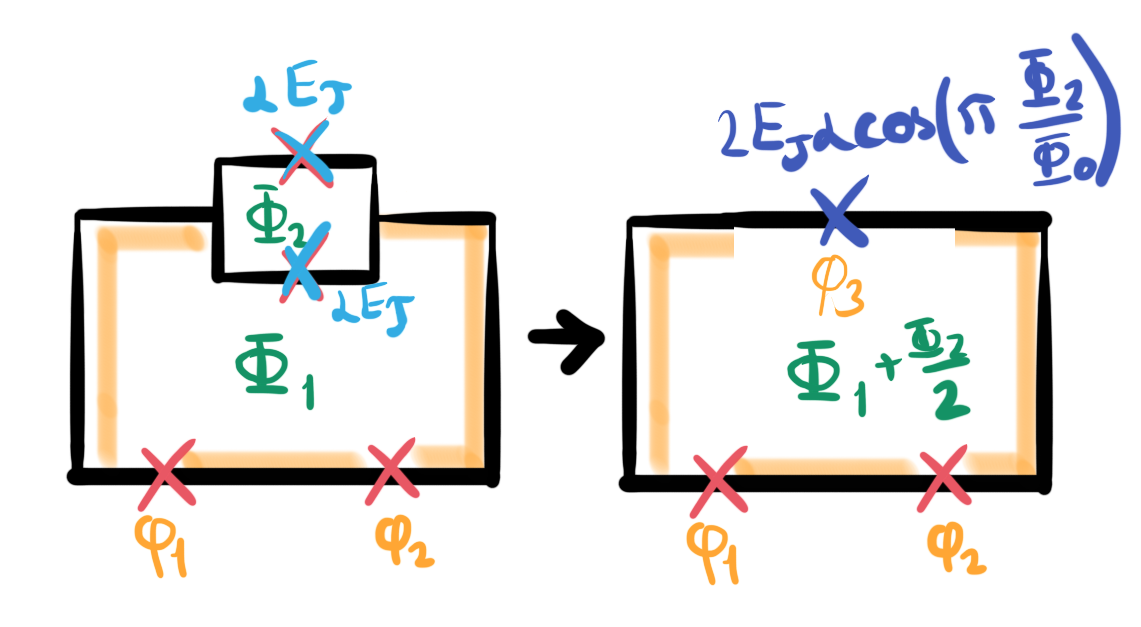
\includegraphics[height=7cm]{flux_4jj_1}
\end{figure}

\begin{enumerate}
\item   The    two   JJ's    of   SQUID    come   together    like   in
  Chapter~\ref{subsec:cpb_2} to create a single Josephson junction with
  a tuneable energy:

  \begin{equation}
    \begin{aligned}
      E_{SQUID} & = \frac{\Phi_0I_c}{2\pi}\times 2|\cos(\pi\Phi_\text{2}/\Phi_0)|\\
      & \equiv E_J \times \green{2|\cos(\pi\Phi_\text{2}/\Phi_0)|}.
    \end{aligned}
  \end{equation}

\item The effective flux penetrating the full loop is

  \begin{equation}
    \Phi_\text{total} = \Phi_1 + \frac{1}{2}\Phi_2.
  \end{equation}

  \noindent One can  think of the flux  in the SQUID loop,  $ \Phi_2 $,
  affecting the lower one only through one of the JJ.

\item    \red{\textbf{The    potential    energy}}   of    the    terms
  $ 1  - \cos(\phi_{ij}) $  of the JJ's  around the circuit  (using the
  quantisation                                                condition
  \purple{$ \phi_3  - \phi_1 +  \phi_2 -  2\pi f_\text{total} =  2\pi n
    $}):

  \begin{equation}
    U_\text{potential} = E_J \bigg[2 + 2\alpha - \cos(\phi_1) - \cos(\phi_2) - \green{2\cos(\pi f_2)}\cos\big(\purple{\phi_1 - \phi_2 + 2\pi(f_1+\frac{1}{2}f_2)}\big) \bigg].
  \end{equation}

  \noindent And this is what it looks like:
  \begin{figure}[h]
    \centering 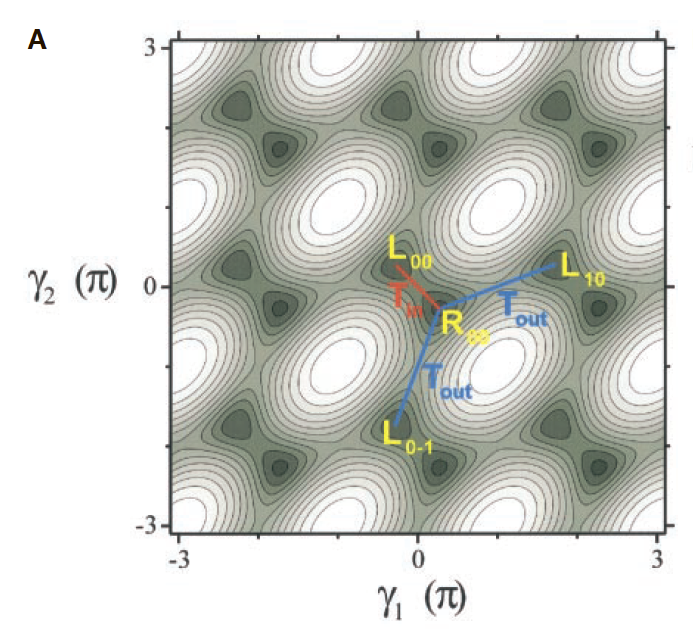
\includegraphics[height=8cm]{flux_4jj_2}
  \end{figure}

  \noindent  circulate in  the  same  direction, state  $  R  $ in  the
  opposite.   The  link  between   the  states  depends  on  parametesr
  $ \alpha $ and $ f_2 $.

\item\
  \begin{framed}\noindent
    \red{If $  f_1+\frac{1}{2}f_2 = 1  $, we recover the  3JJ potential
      from Chapter~\ref{subsec:l33jj}.}
  \end{framed}

\item \textbf{\red{The kinetic energy}} is harder to evaluate.

  \begin{equation}
    \left\lbrace \begin{aligned}
        \vec{V} & = 2eC^{-1}\vec{n}\\
        \vec{Q} & = 2e\vec{n}\\
        \red{U_{\text{kinetic}}} & \red{= \frac{1}{2}Q.V}\\
      \end{aligned}\right.  \Rightarrow \red{U_{\text{kinetic}} =
      \frac{1}{2}\left(2e\vec{n}^{\text{T}}\right)\left(2eC^{-1}\vec{n}\right)
      = \frac{(2e)^2}{2}\vec{n}^{\text{T}}C^{-1}\vec{n}},
  \end{equation}

  \noindent where $ \vec{n}  $ is the charge state on  the 3 islands in
  the  system and  $  C $  is  the capacitance  matrix  for the  system
  (confusingly, the  capacitance for  JJ's 1  and 2  is also  given the
  symbol $ C $).

  \begin{framed}\noindent
    \noindent \textbf{It is common  to work classical analogues}, where
    we would write:
    \begin{equation}
      \frac{(2e)^2}{2}\vec{n}^{\text{T}}C^{-1}\vec{n} = \frac{1}{2}\vec{p}^{T}M^{-1}\vec{p}.
    \end{equation}

    \noindent  $ M  $  is  the mass  tensor,  with nornalisation  value
    $    \hbar^2/\frac{(2e)^2}{2C}   $,    where   we    have   applied
    $ \icommutation{x}{p}=i\hbar $  and $ \icommutation{\phi}{n} =  i $ to
    generate the $ \hbar $.

  \end{framed}

\begin{framed}\noindent
  Depending on the  direction that we are looking  at tunneling across,
  we get two tensors:
  \begin{itemize}
  \item $ M_a  = \frac{1}{4}M$ for the $ \phi_1-\phi_2  = 0 $ direction
    \hfill (across the tall barrier);
  \item $  M_b =  M$ for  the $  \phi_1+\phi_2 =  0 $  direction \hfill
    (across the snall barrier);
  \end{itemize}
\end{framed}

\item  The result  it two  different transistions,  with two  different
  oscillation frequencies.

\item \red{\textbf{Make sure barrier is high enough, to localise state,
      and small enough to allow sufficient tunneling to occur.}}
\end{enumerate}
